\RequirePackage[l2tabu,orthodox]{nag}
\RequirePackage{fixltx2e}

\documentclass{beamer}

% bunch of special fonts for various symbols
\usepackage{mflogo}
\usepackage{manfnt}
\usepackage{hieroglf}
\usepackage{marvosym}
\usepackage{wasysym}

% typeset URLs properly, in sans serif
\usepackage{url}
\urlstyle{sf}

% except for the TeX logos this looks better
\usepackage[defaultsans]{droidsans}

% some additional beamer customization
\setbeamertemplate{navigation symbols}{}
\setbeamertemplate{itemize/enumerate subbody end}{\vspace{\baselineskip}}

\usefonttheme{structurebold}

\usecolortheme{whale}
\usepackage{jhcolors}
\setbeamercolor{structure}{fg=jhazure}

% command to produce sectioning slides
\newcommand{\cutesection}[2]{
  \section{#1}
  \frame{
    \frametitle{#1}
    \begin{center}
      \Huge{#2}\\\textbf{#1}
    \end{center}
  }
}

% start of presentation proper
\title{A Brief Intro to \LaTeX{} and Friends}
\author{Peter H.\ Fr{\"o}hlich\\
{\footnotesize phf@cs.jhu.edu}}
\date{February 12, 2015}

\begin{document}

\frame{
  \titlepage
}

\frame{
  \frametitle{Outline}
  \tableofcontents
}

\cutesection{Motivation}{\smiley}

\frame{
  \frametitle{Cute Mascot!}
  \begin{center}
    
\includegraphics[height=0.8\textheight]{lion}\\
    {\tiny\url{http://www.ctan.org/lion/}}
  \end{center}
}

\frame{
  \frametitle{Seriously, why \LaTeX{}?}
  \begin{itemize}
    \item Standard in Computer Science and related disciplines.
    \begin{itemize}
      \item Your (future?) co-authors (will!) use it already.
      \item Most conferences accept it cheerfully.
      \item Some conferences actually require it.
    \end{itemize}
    \item Documents in plain text format (for the most part).
    \begin{itemize}
      \item Straightforward for versioning systems.
      \item Trivially portable (but avoid funky encodings!).
      \item Easily generated from stuff like Markdown.
    \end{itemize}
  \end{itemize}
}

\frame{
  \frametitle{Seriously, why \LaTeX{}?}
  \begin{itemize}
    \item Integrated ``well enough'' with the command line.
    \begin{itemize}
      \item Use your favorite build system.
      \item Integrate with whatever else you need.
      \item Produce complex documents automatically.
    \end{itemize}
    \item Extensible with macros and packages.
    \begin{itemize}
      \item Use macros to customize ``little things'' in documents.
      \item Develop your own classes to standardize documents.
      \item Packages for anything from musical scores to chess games.
    \end{itemize}
  \end{itemize}
}

\cutesection{History}{\textpmhg{\Ha\Hv\Hman}}

\frame{
  \frametitle{Donald Knuth}
  \begin{center}
    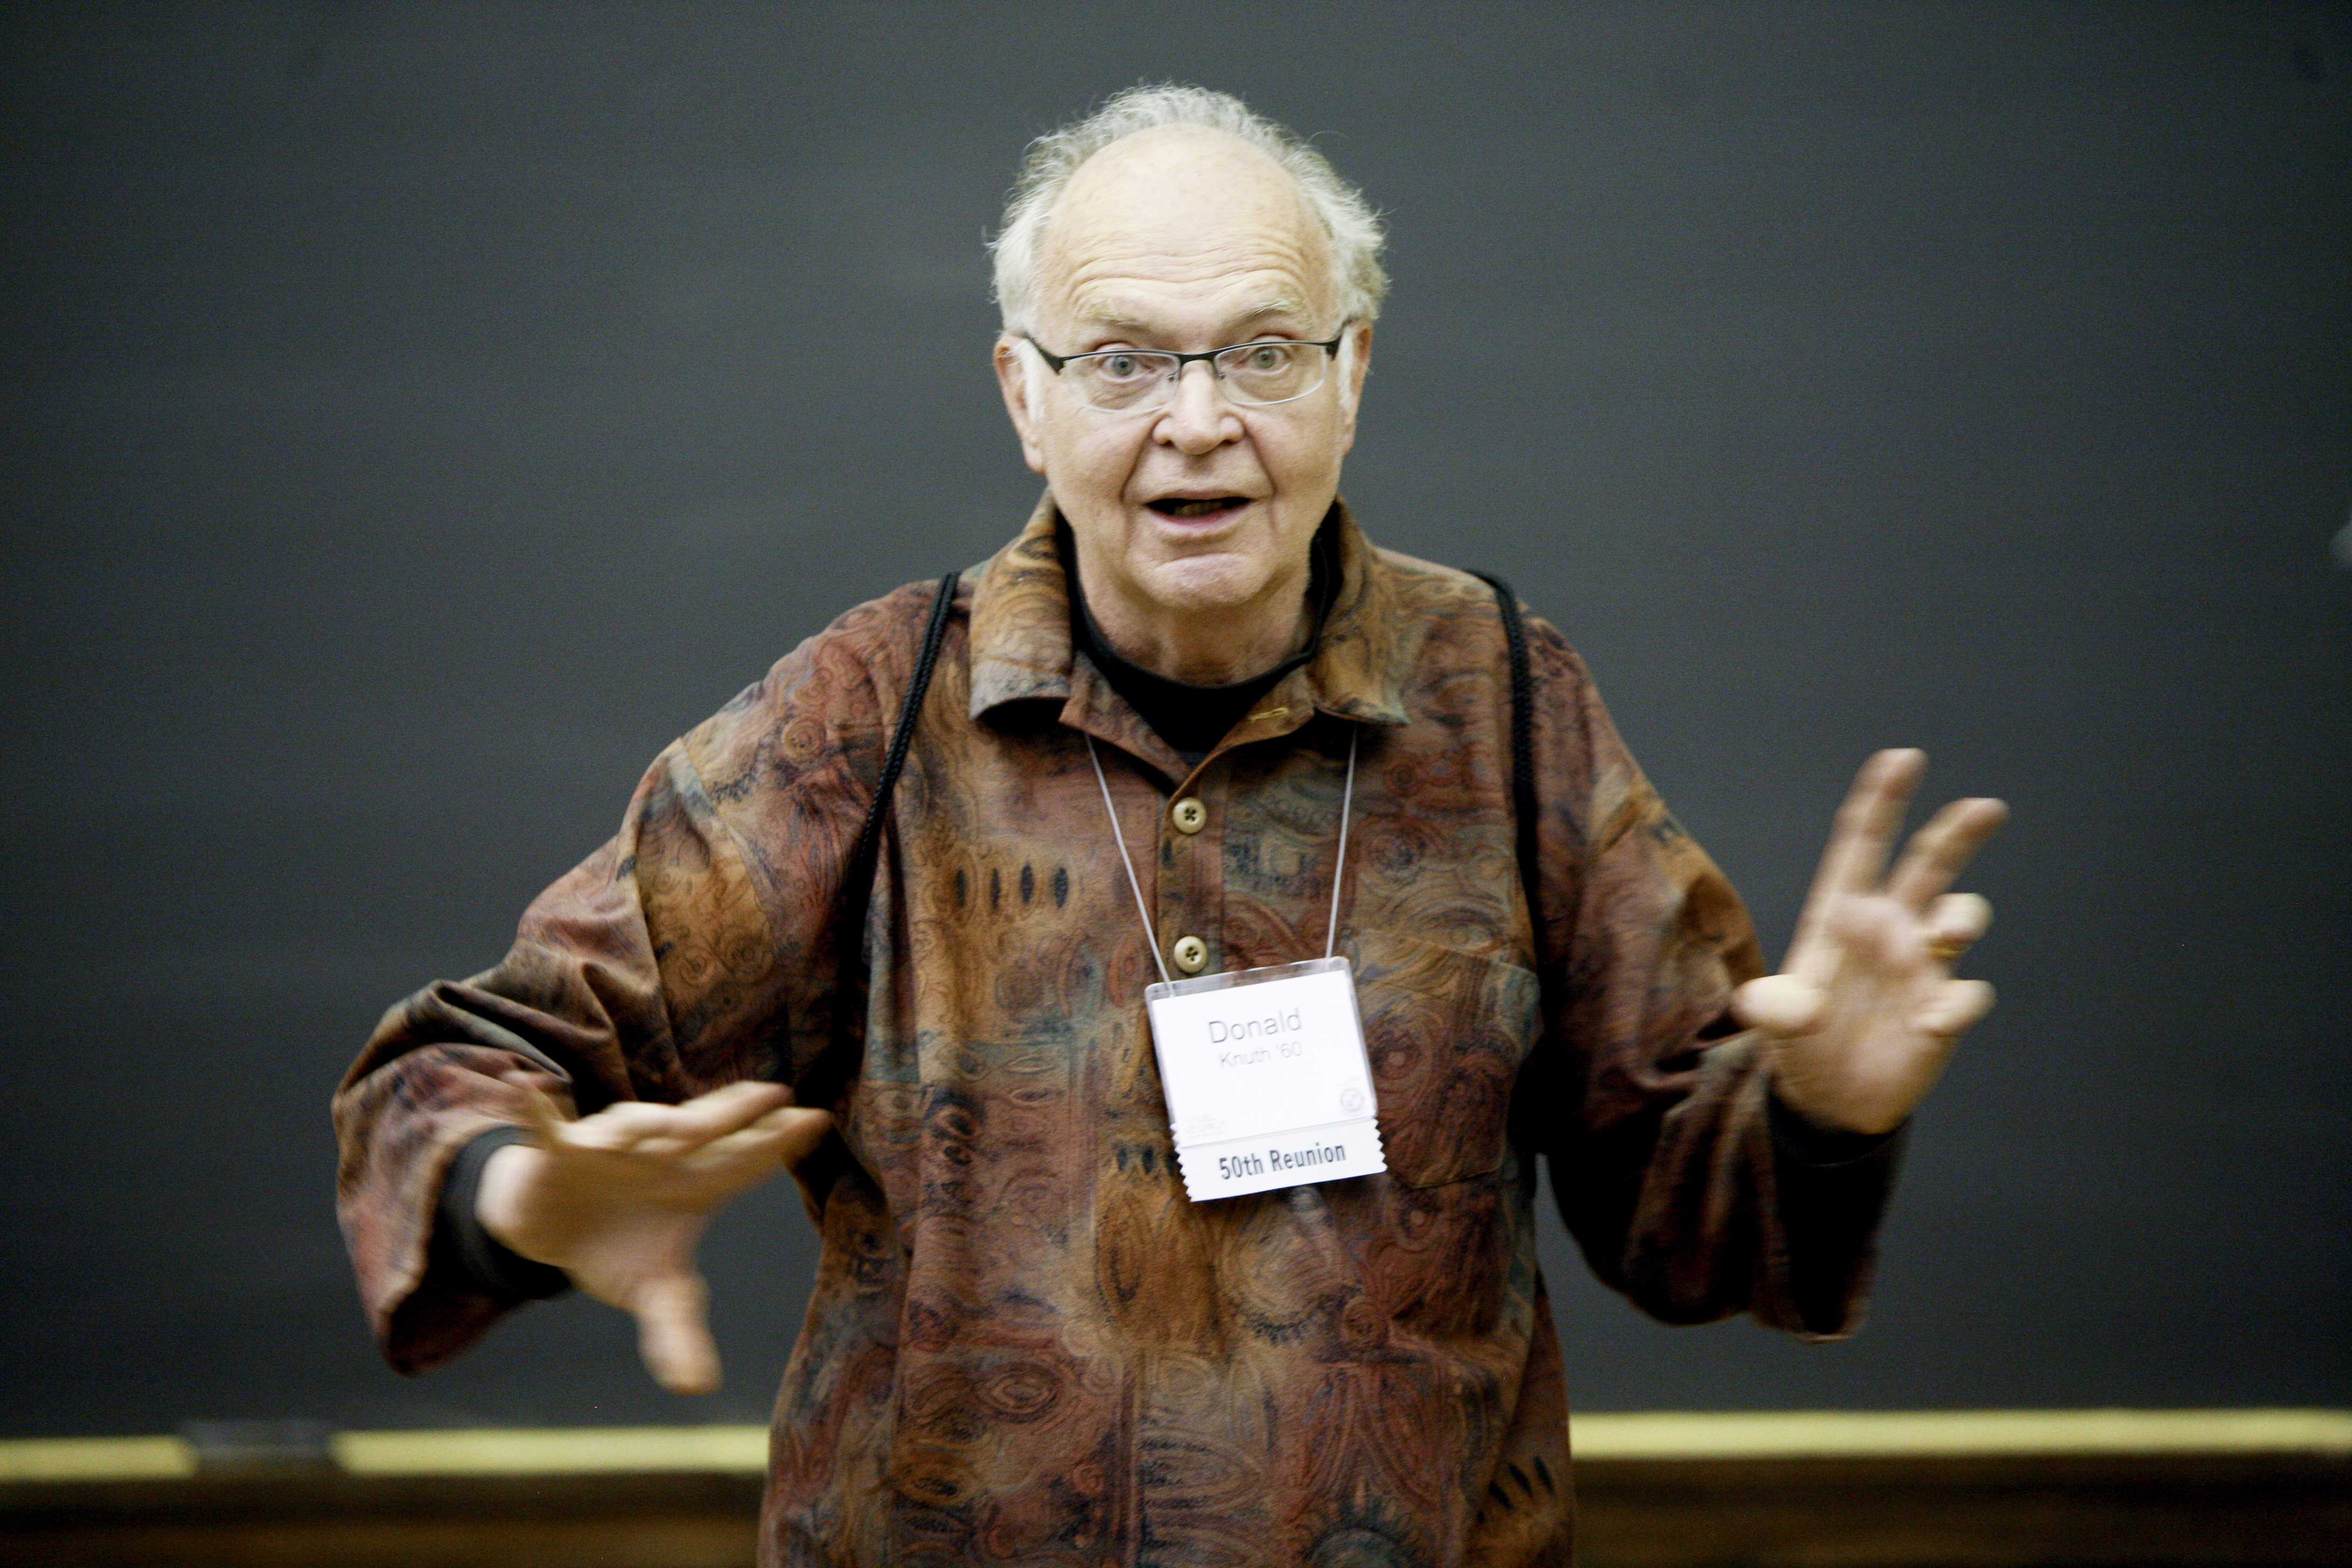
\includegraphics[width=\textwidth]{knuth}\\
    {\tiny\url{http://www-cs-faculty.stanford.edu/~uno/graphics.html}}
  \end{center}
}

\frame{
  \frametitle{Donald Knuth}
  \begin{itemize}
    \item ACM Turing Award (1974)
    \begin{itemize}
      \item \emph{For his major contributions to the
        analysis of algorithms and the design of
        programming languages\dots}
    \end{itemize}
    \item Wanted to produce beautiful books, by himself.
    \begin{itemize}
      \item Studied typography and font design, in depth.
      \item Interesting algorithms, for example hyphenation.
      \item Developed \TeX{} and \MF{} languages and tools.
      \item Documented (with complete source) in five books.
    \end{itemize}
    \item Version numbers converge to \(\pi\) and \(e\) on Knuth's death.
    \begin{itemize}
      \item \emph{\dots{}all ``bugs'' will be permanent ``features.''}
      \item Designed for ``eternity,'' not necessarily ``modernity.''
    \end{itemize}
  \end{itemize}
}

\frame{
  \frametitle{Leslie Lamport}
  \begin{center}
    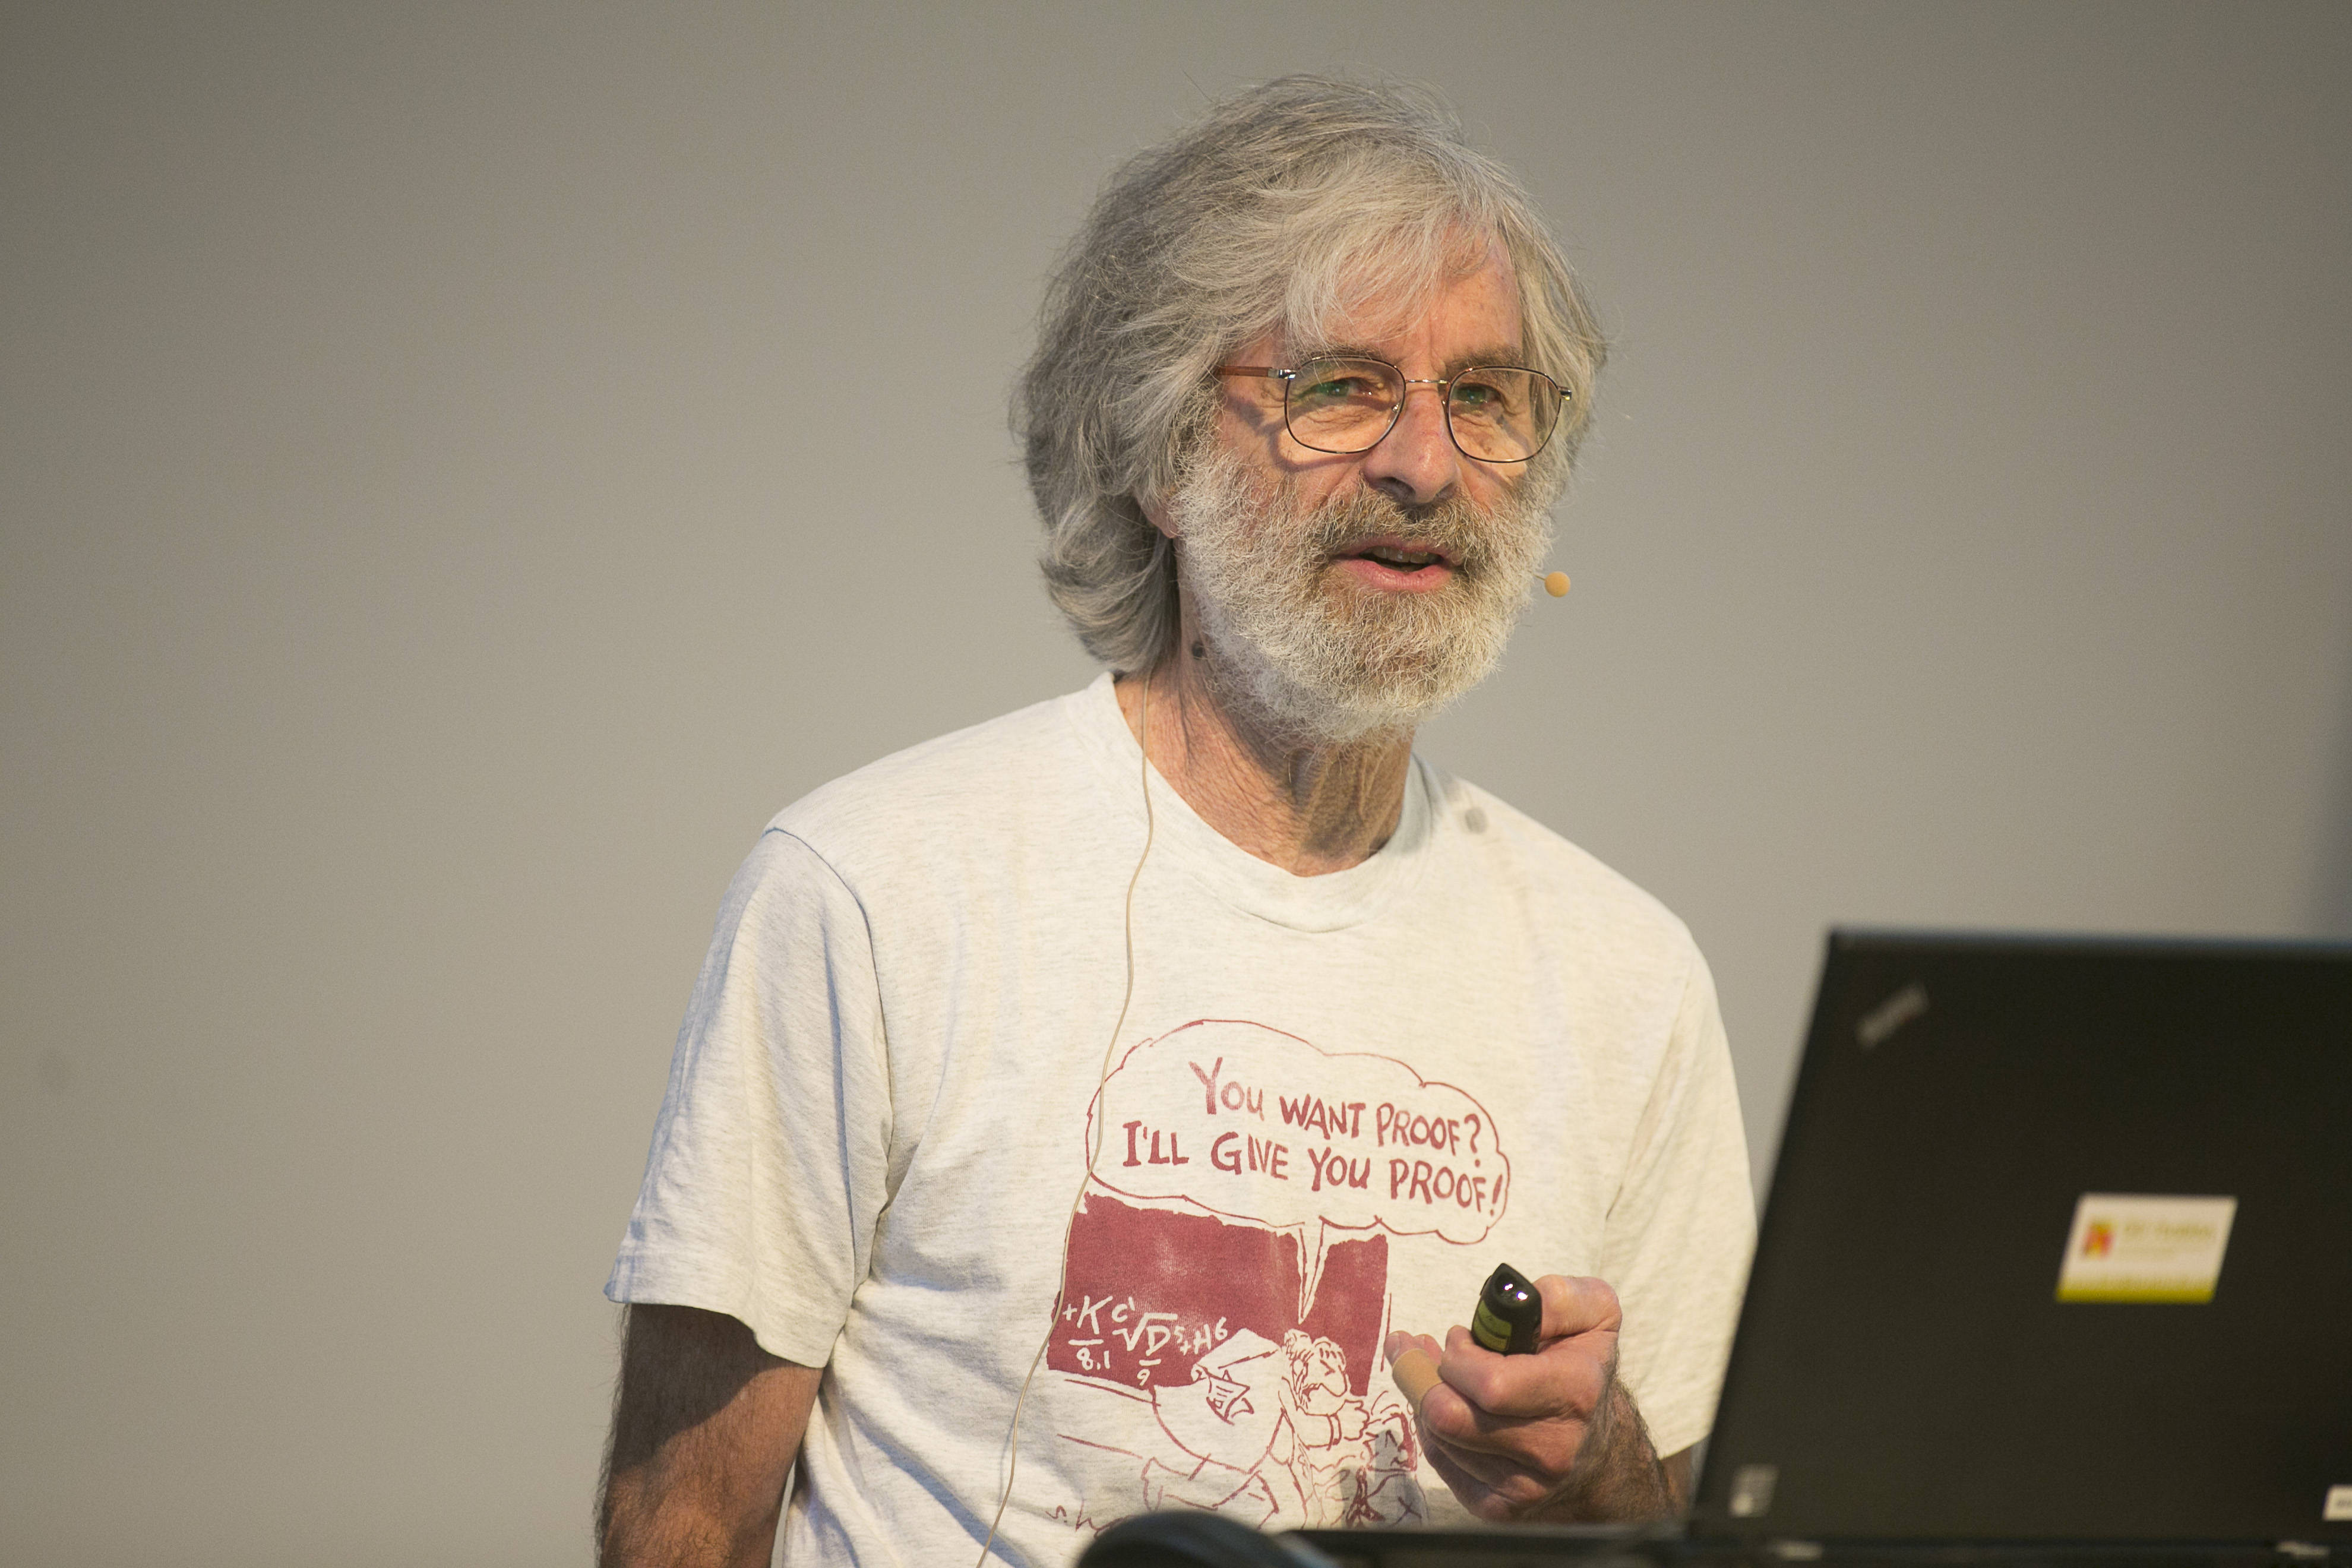
\includegraphics[width=\textwidth]{lamport}\\
    {\tiny\url{http://www.scilogs.com/hlf/writing-for-mathematical-clarity/}}
  \end{center}
}

\frame{
  \frametitle{Leslie Lamport}
  \begin{itemize}
    \item ACM Turing Award (2013)
    \begin{itemize}
      \item \emph{For fundamental contributions to the
        theory and practice of distributed and
        concurrent systems\dots}
    \end{itemize}
    \item Wanted to use \TeX{} to write a book on concurrency.
    \begin{itemize}
      \item Found \TeX{} too low-level, wanted more structure.
      \item Developed \LaTeX{} macro package to that end.
      \item Never wrote that concurrency book\dots{}
      \begin{itemize}
        \item Did write a \LaTeX{} book however! \smiley
      \end{itemize}
    \end{itemize}
    \item Since taken over by a ``cast of thousands'' as it were.
    \begin{itemize}
      \item Quite different from Lamport's original if you look closely.
      \item Also emphasizes stability and backwards-compatibility.
    \end{itemize}
  \end{itemize}
}

\cutesection{Caveats}{\textdbend}

\frame{
  \frametitle{Caveats}
  \begin{itemize}
    \item \LaTeX{} can be a bit frustrating when you start out.
    \begin{itemize}
      \item Just trust that once you get it, you won't go back.
      \item Keep it simple, focus on content not presentation.
      \item Google (or whatever search engine) is your friend.
    \end{itemize}
    \item There's a huge ecosystem out there!
    \begin{itemize}
      \item Almost everything exists (but it might be 20 years old).
      \item Can be difficult to find exactly what you're looking for.
      \item Luckily it's generally a pretty friendly community.
    \end{itemize}
  \end{itemize}
}

\frame{
  \frametitle{Caveats}
  \begin{itemize}
    \item Packages may seem like modules, but they are really not.
    \begin{itemize}
      \item Subtle interactions between different packages.
      \item Order of ``import'' can matter even though it shouldn't.
      \item It's almost all text-macros in the end, act accordingly!
    \end{itemize}
    \item Use all the tools at your disposal to limit problems.
    \begin{itemize}
      \item Keep it simple, baby steps, RTFM, \dots{} you know the drill.
      \item Always use \texttt{fixltx2e} and \texttt{nag} as I'll show you!
      \item Actually pay attention to the darn warnings?
    \end{itemize}
  \end{itemize}
}

\cutesection{Demo}{\Keyboard{} \ComputerMouse}
\cutesection{Questions?}{\frownie}

\end{document}
